%% IJCAS regular paper (6-10 pages, two-column; IJCAS.cls from the 2026-02-19 template)
%% Revised draft v0.2 (2026-11-05). Red \tbd{} = placeholder for results that are still running (see docs/EXPERIMENTS.md)
%% or facts to verify. Figures: paper/figs/*.pdf (python paper/make_figs.py).
\documentclass{IJCAS}

\usepackage{url}
\usepackage{array,tabularx}
\usepackage{multicol}
\usepackage{multirow}

\newcommand{\tbd}[1]{\textcolor{red}{[#1]}}
\newcommand{\note}[1]{\texttt{\small #1}}
\newcommand{\pizf}{$\pi_{0.5}$}

%%%% Editorial Information (do not modify)
\journalvolumn{VV}
\journalnumber{X}
\journalyear{YYYY}
\setarticlestartpagenumber{1}

\setlength{\headheight}{14.5pt}
\allowdisplaybreaks

\begin{document}

\title{Event-Driven Language Memory for Long-Horizon Vision-Language-Action Policies}

\author{\tbd{Author names}*}

\begin{abstract}
Manipulation under partial observability requires a policy to retain cues that are absent when the relevant action is executed.
We investigate whether an external language memory can supply this information to a vision-language-action (VLA) policy without changing its architecture.
Our pipeline detects visual changes while the robot is stationary, captions the pre-change region, and appends short notes to the instruction of a fine-tuned $\pi_{0.5}$ policy.
On RememberColor3/5/9-Long, notes increase success from 0.14/0.14/0.08 to 0.96/0.94/0.49 under matched demonstration and policy-training budgets; an oracle-conditioned policy reaches 0.87 on the nine-color task.
We examine this gap through memory selection, attribute representation, and policy utilization.
Changing the note writer at test time changes the success of a fixed policy by up to 24 percentage points, although the intervention changes both content and format.
Measured color names reduce similar-color target confusions from 13 to 5 of 50 episodes, without improving aggregate nine-color success.
Correct cue notes can still lead to incorrect target choices, exposing a limitation beyond note accuracy.
Across a custom set of 26 long-horizon tasks, benefits concentrate on single-cue object recall; multi-cue, tracking, counting, and timing tasks remain difficult.
An event-matched tiled visual-memory baseline provides no consistent improvement under the tested budget.
These results identify both the value and the limits of short language notes as an interface between past observations and current VLA decisions.
\end{abstract}

\begin{keywords}
Long-horizon manipulation, memory, partial observability, robot learning, vision-language-action models.
\end{keywords}

\maketitle

\makeAuthorInformation{
\tbd{Manuscript received ...; affiliations; e-mails.}\\

* Corresponding author.
}

\runningtitle{2026}{\tbd{Authors}}{Event-Driven Language Memory for Long-Horizon Vision-Language-Action Policies}{xxx}{xxxx}{x}


%======================================================================
\section{INTRODUCTION}
%======================================================================
Many manipulation tasks are partially observable in time: the information that determines the correct action is shown once and is no longer visible when the action must be taken.
A robot that is shown a colored cube, waits while the cube is removed, and must later touch the cube of the same color among several candidates cannot solve the task from its current camera image alone.
In the current-observation configuration studied here, $\pi_{0.5}$~\cite{pi05} maps camera images, proprioception, and an instruction to an action chunk, without an explicit persistent observation memory. This configuration cannot directly recover a cue that is absent from its inputs.
On our custom set of 26 long-horizon tasks, this policy reaches a mean success rate of 0.048 at the final 90k-step checkpoint.

Recent work adds memory to VLA policies in several forms: latent memory banks~\cite{memoryvla,memoryvlapp}, recurrent memory tokens inside the backbone~\cite{muvla}, visual keyframes selected when the action plan changes~\cite{replanmem}, and histories of past frames~\cite{simplememvla}.
These approaches change what the policy sees, but it remains difficult to tell \emph{why} a memory-augmented policy fails: because the relevant information was never written, because it was written in a form the policy cannot use, or because the policy does not act on correct information.
Language memory makes these questions measurable.
A text note can be read, replaced by the ground truth, or edited at test time without retraining, so each stage can be tested in isolation.
RoboMME~\cite{robomme} observed that VLM-written language subgoals reach only about a third of the success obtained with ground-truth subgoals; our goal is to understand and reduce such a gap.

We present an event-driven language memory for VLA policies (Fig.~\ref{fig:pipeline}).
A detector fires when a part of the scene changes while the robot is still, the changed region is cropped and described by a small vision-language model, and only the content that \emph{disappeared} is kept as a short note such as \note{Gone: a aqua cube.}
The notes are appended to the instruction string; the policy architecture and action-learning objective are unchanged, while its instruction is augmented with memory.
We analyze the pipeline along three axes: \emph{selection} (when and what to write), \emph{representation} (in which words), and \emph{utilization} (whether the policy acts on the note).

Our contributions are:
\begin{itemize}
\item An external event-note pipeline that supplies disappeared visual cues through the existing VLA instruction interface, without modifying the policy architecture.
\item Fixed-policy note interventions and target-choice diagnostics that distinguish sensitivity to note content from failures despite correct cue descriptions.
\item An analysis of the gap between memory correctness and action success using generated notes, oracle notes, content-swapped notes, and visual memory.
\item An evaluation on 26 long-horizon memory tasks with one joint policy per method, characterizing where lightweight language memory helps and where it does not, with supplementary short-task results and published baselines provided as protocol-dependent context.
\end{itemize}

%======================================================================
\section{RELATED WORK}
%======================================================================
\subsection{Memory-augmented VLA policies}
MemoryVLA~\cite{memoryvla} and MemoryVLA++~\cite{memoryvlapp} maintain perceptual and cognitive memory banks queried by a diffusion action expert. $\mu$VLA~\cite{muvla} adds recurrent memory tokens to a pretrained VLA backbone. SimpleMemVLA~\cite{simplememvla} provides a timestamped visual history to a video-capable backbone. Non-VLA visuomotor policies with memory include GMP~\cite{gmp} and Chameleon~\cite{chameleon}. These methods report results on the standard MIKASA-Robo RememberColor tasks~\cite{mikasa} with different backbones, training sets, and checkpoint selection; we therefore compare against our own baselines under identical conditions and list published numbers only for reference.

\subsection{Event-driven memory selection}
RePlanMem-VLA~\cite{replanmem} writes a visual keyframe when overlapping action-chunk predictions disagree and evaluates the detection and retention of memory-relevant frames on MIKASA-Robo-VLA. Our trigger is an observation change rather than a plan change, and we store a text description of the removed content rather than the frame. We evaluate a tiled-keyframe baseline inspired by this representation, using our trigger rather than reproducing its plan-based selection (Section~\ref{sec:setup}).

\subsection{Language memory for robot policies}
RoboMME~\cite{robomme} benchmarks fourteen memory variants on top of $\pi_{0.5}$ and finds that language subgoals are strong when accurate (84\% with oracle subgoals) but weak when generated by a VLM (33\%). We study the same kind of gap for event notes and attribute it to selection, representation, and utilization.

\subsection{Benchmarks}
MIKASA-Robo~\cite{mikasa} evaluates memory-dependent manipulation. Its language-conditioned extension, MIKASA-Robo-VLA~\cite{mikasavla}, provides 90 tasks and 250 demonstrations per task. The reference $\pi_{0.5}$ policy of~\cite{mikasavla}, fine-tuned on 14 tasks, reaches a mean success of 0.211.

%======================================================================
\section{METHOD}
\label{sec:method}
%======================================================================
\begin{figure*}[!t]
\centering
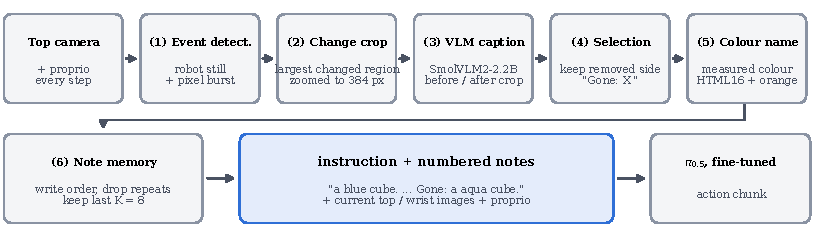
\includegraphics[width=\textwidth]{figs/fig_pipeline.pdf}
\caption{Event-driven language memory. Notes are written only at change events, only for the content that disappeared, and are appended to the instruction of an unmodified $\pi_{0.5}$ policy. The same pipeline labels the training demonstrations and runs online at test time.}
\label{fig:pipeline}
\end{figure*}

The policy is $\pi_{0.5}$~\cite{pi05} fine-tuned with LeRobot~\cite{lerobot}. Its observations are a top and a wrist camera image ($128\times128$) and the proprioceptive state, and memory enters only through the instruction string. At every step the policy receives
\begin{center}
\note{\{instruction\} Notes: (1) $n_1$ (2) $n_2$ \dots}
\end{center}
where $n_1, n_2, \dots$ are the notes written so far. The same pipeline is applied to the demonstrations to build the training instructions and runs online during evaluation.

\subsection{Event detection}
Let $I_t$ be the top-camera image and $q_t$ the full proprioceptive vector. Define the changed-pixel count
\begin{equation}
c_t=\sum_{u,v}\mathbf{1}\!\left[\max_j|I_t(u,v,j)-I_{t-1}(u,v,j)|>40\right].
\end{equation}
With a history of up to $W=5$ previous steps, a change event requires (i) every recorded proprioceptive increment in that history, including the current increment, to have infinity norm below $10^{-3}$; (ii) $c_t\geq8$; and (iii) $c_t\geq4(1+\operatorname{median}(c_{t-W},\ldots,c_{t-1}))$, using the available nonempty history near episode start.
The stationarity threshold is applied componentwise in the proprioceptive vector's native units.
This rule suppresses, but cannot eliminate, changes associated with robot motion and uses no task label.
We retain the frame before the first change and accumulate masks over a burst.
A note is written when fewer than eight pixels change or after five subsequent steps without a new event; a new event restarts this settling counter.
The first frame is handled separately as a scene-note event.
During CPU evaluation, arm action components are zeroed when their maximum absolute value is below 0.02, leaving the gripper command unchanged. This dead band is shared across the matched methods and reduces drift during waiting periods.

\subsection{Change localization}
We intersect the accumulated change mask with changes that persist between the pre-event and settled images, dilate it by four iterations to group nearby pixels, and retain the component containing the most original changed pixels. Regions with fewer than four persistent pixels are discarded. A square crop around it is taken from the frames before and after the event and upsampled to $384\times384$ with nearest-neighbor interpolation. A cue cube that covers $3\times3$ pixels of the $128\times128$ camera becomes legible to the captioner, while the crop reduces the surrounding context that can distract the captioner. Background pixels and captioning errors can still enter the note.

\subsection{Captioning and selection}
SmolVLM2-2.2B~\cite{smolvlm} captions the before and after crops separately with the prompt \emph{``List the objects in the image with precise color names, e.g. `a cyan cube, a maroon cube'. The wooden surface is not an object. If there are no objects, answer `nothing'.''}
Captioning the two crops jointly was unreliable about which content appeared and which disappeared.
Content that appeared remains visible to the policy and is therefore not stored.
The before caption is used as a proxy for disappeared content, rather than an object-level set difference. Only this side is kept, as \note{Gone: X.}, and notes whose $X$ is empty or the table surface are dropped.
A scene note of the full first frame is written once at $t=0$.

\begin{figure*}[!t]
\centering
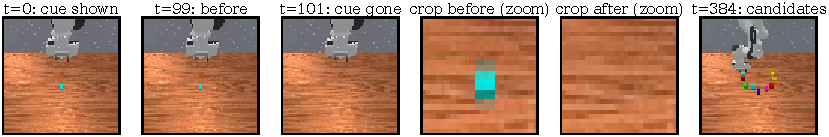
\includegraphics[width=\textwidth]{figs/fig_example.pdf}
\caption{Notes written for a RememberColor9-Long demonstration (cue: aqua cube). The change between $t=99$ and $t=101$ triggers an event; the zoomed crops show the removed cue. v3: \note{Change: a cyan cube, a maroon cube -> brown.} (the captioner splits the shaded faces into two objects); v4: \note{Gone: a cyan cube, a maroon cube.}; v6: \note{Gone: a aqua cube.} At the decision the v6 policy receives \note{Observe the cube's color, wait, then touch the cube of the same color. Notes: (1) a blue cube. (2) Gone: a aqua cube.}}
\label{fig:example}
\end{figure*}

\subsection{Representation}
The captioner identifies color families reliably but uses one name for pairs such as maroon and red, orange and yellow, or teal and cyan.
We therefore replace the first color word of a note by a measured name: the mean RGB of persistent changed pixels in the pre-event image whose channel range ($\max(R,G,B)-\min(R,G,B)$) is at or above its 75th percentile, mapped by squared Euclidean RGB distance to the nearest of the 16 HTML basic colors plus orange. Ties at the percentile can include more than 25\% of the pixels.
A coarse, standard vocabulary keeps the measured name stable between the demonstrations and the online rollouts; a finer vocabulary (148 CSS colors) produced different names for the same cue under small rendering differences.
Only the first object of a note is kept, because the captioner occasionally describes the shaded top and side faces of one cube as two objects (Fig.~\ref{fig:example}).

\subsection{Note memory and training}
Notes are kept in write order; the burst-settled v3--v7 writers do not apply additional burst merging. A note identical to the previous one is dropped, and the last $K=8$ notes are appended to the instruction.
For training, the instruction of every demonstration frame contains the notes written up to that frame, and $\pi_{0.5}$ is fine-tuned on these instructions with the standard objective and hyperparameters.

%======================================================================
\section{EXPERIMENTAL SETUP}
\label{sec:setup}
%======================================================================
\subsection{Tasks}
We use the \emph{Long} variants of MIKASA-Robo-VLA~\cite{mikasavla}, in which the cue is followed by a delay of 50--450 steps before the decision. The main analysis uses RememberColor3/5/9-Long (RC3/5/9-L): a cue cube is shown, removed, and after the delay 3, 5, or 9 candidate cubes appear; the robot must touch the one with the cue color. The generality study uses all 26 environments whose names carry the \texttt{-Long} suffix (Table~\ref{tab:long}), which cover object, capacity, sequential, tracking, and temporal memory. This is a custom subset: by the official split, 14 of them belong to the long and 12 to the medium split, and the official long tasks BatteriesChecker, TraceShapeSeq, and GatherAndRecall are not included.

\subsection{Physics backend}
The demonstrations of these tasks were collected by a motion planner with the CPU physics backend. Replaying the recorded actions with the original seeds succeeds in 8/8 episodes on the CPU backend and 0/8 on the GPU backend used by the canonical evaluation, with trajectory deviations of 2.5--4.5\,cm. Different inverse-kinematics behavior is a suspected contributor; the replay check does not isolate the source of the backend discrepancy. We therefore evaluate on the CPU backend, consistent with the data.

\subsection{Training and evaluation}
\begin{table}[!t]
\caption{Protocol for the main Long-task experiments. Short-task differences are specified in their table captions.}
\label{tab:setup}
\begin{center}
{\footnotesize
\resizebox{\columnwidth}{!}{%
\begin{tabular}{ll}
\hline
Policy & $\pi_{0.5}$ (\texttt{pi05\_base}), LeRobot, bf16 \\
Inputs & top + wrist RGB $128\times128$, proprioception \\
Actions & chunk 10, execute 5, end-effector delta pose \\
Data & 250 demonstrations per task \\
Training & joint over a task set, batch 16 \\
 & RC-L (3 tasks): 20k steps; Long-26: 90k steps \\
Evaluation & 50 episodes per task, fixed seeds \\
 & RC9-L: 150 episodes for the main models \\
Checkpoint & RC-L: final 20k; Long-26: matched 45k,\\
 & final 90k also reported for no memory and v6 \\
Physics & CPU backend (matches demonstrations) \\
Metrics & success; for RC tasks also the approached cube \\
\hline
\end{tabular}}
}
\end{center}
\end{table}
Table~\ref{tab:setup} summarizes the protocol. Checkpoint configurations specify AdamW with learning rate $2.5\times10^{-5}$, $\beta=(0.9,0.95)$, $\epsilon=10^{-8}$, weight decay 0.01, and gradient clipping at norm 1.0. The configured scheduler uses 1,000 warmup steps and 30,000 decay steps toward $2.5\times10^{-6}$. One policy is trained jointly per task set and method, using one training seed per configuration. Evaluation seeds are $4242424242+i$ for episode index $i$, shared across methods; the 150-episode RC9-L evaluation extends the first 50 episodes. Online images undergo YUV420 chroma subsampling to match demonstration-video color degradation. Success is the environment \texttt{success\_once} indicator. We report Wilson 95\% intervals for the extended RC9-L evaluation; these quantify episode uncertainty conditional on a trained checkpoint, not variation across training seeds. We additionally report paired percentile-bootstrap intervals for selected success differences (20,000 resamples of matched episode seeds, bootstrap RNG seed 20261105; no multiplicity correction). For RememberColor we record the cube with the smallest gripper distance over the rollout as a target-choice proxy. This diagnostic is distinct from the environment success condition and need not identify every cube contacted during a trajectory.

\subsection{Compared methods}
Within each matched comparison, methods share demonstration trajectories, policy-training steps, evaluation seeds, and control settings. Memory construction and its associated computation differ; equal policy-training steps do not imply equal total compute.
\begin{itemize}
\item \textbf{No memory}: the original instruction.
\item \textbf{Notes v2--v6}: successive versions of our pipeline (Table~\ref{tab:rc}). v2 captions the full frame with SmolVLM2-500M at each event; v3 captions zoomed before/after crops as \note{Change: X -> Y.}; v4 keeps only the removed side (selection); v5 and v6 add measured color names with a fine (148) and a coarse (17) vocabulary (representation).
\item \textbf{v7}: v6 without the scene note at $t=0$.
\item \textbf{Visual memory}: the zoomed crops (\emph{crop}) or full frames (\emph{keyframe}, inspired by RePlanMem-VLA~\cite{replanmem}) written at our events are stored in a $3\times3$ grid of $42\times42$ tiles in an additional $128\times128$ camera image. The grid retains the first nine writes. This baseline tests this particular compressed visual interface; it is not a reproduction of RePlanMem-VLA.
\item \textbf{Oracle note}: a cue color label appended to the instruction using a separate oracle-labeling pipeline. This is a privileged reference, not a formal upper bound: its wording and cue availability differ from event notes.
\end{itemize}

%======================================================================
\section{RESULTS AND ANALYSIS}
%======================================================================
\subsection{Main result on RememberColor-Long}
\begin{table}[!t]
\caption{Success rate on RememberColor-Long (one joint policy per row, 20k steps, 50 episodes per task; RC9-L also with 150 episodes and Wilson 95\% CI).}
\label{tab:rc}
\begin{center}
{\footnotesize
\setlength{\tabcolsep}{4pt}
\begin{tabular}{lcccc}
\hline
Memory & RC3-L & RC5-L & RC9-L & RC9-L ($n{=}150$) \\
\hline
None & 0.14 & 0.14 & 0.06 & 0.08 [0.05, 0.13] \\
Visual (crop) & 0.12 & 0.12 & 0.14 & -- \\
Notes v2 & 0.86 & 0.86 & 0.50 & 0.50 [0.42, 0.58] \\
Notes v3 & 0.96 & 0.84 & 0.38 & 0.41 [0.33, 0.49] \\
Notes v4 & 0.94 & 0.90 & 0.54 & 0.49 [0.41, 0.57] \\
Notes v5 & 1.00 & 0.92 & 0.50 & -- \\
Notes v6 & 0.96 & 0.94 & 0.48 & 0.49 [0.41, 0.57] \\
\hline
Oracle note & 0.96 & 0.98 & 0.80 & 0.87 [0.80, 0.91] \\
\hline
\end{tabular}
}
\end{center}
\end{table}
Table~\ref{tab:rc} shows that event notes turn tasks the policy cannot solve into tasks it solves almost perfectly with three and five colors (0.14 to 0.96 and 0.94), and raise the nine-color task from 0.08 to 0.49; for RC9-L, the paired success difference is 0.413 with a 95\% bootstrap interval of [0.327, 0.500].
For context, uniform target selection would yield choice accuracies of 1/3, 1/5, and 1/9; these are not chance success rates because completing a touch adds an execution requirement. The no-memory results show that the tasks remain difficult, but success alone cannot establish random target choice.
The visual crop memory, which contains the same cue image, stays at the no-memory level: inspection of the online memory image confirmed that it was written correctly, but this does not establish that the policy ignores the input. The result shows no consistent benefit from this visual interface under our data and training budget.
The note versions v2, v4, and v6 have overlapping RC9-L episode confidence intervals; these results do not establish either superiority or equivalence, and we therefore analyze how the versions change the \emph{types} of errors rather than claiming that a later version is better.

Since the delay before the decision is drawn per episode, we also binned the episodes by delay (50--183, 184--316, 317--450 steps). We observe no monotonic decrease in note-policy success across the sampled delay bins (RC9-L v6: 0.48, 0.42, 0.57; oracle: 0.86, 0.87, 0.87), as expected from a memory that is written once and kept. With a fixed delay of 1000 steps, more than twice the longest delay seen in training, the five-task mean is similar: averaged over RC3/5/9-L, Shape3-L, and ShapeAndColor3x2-L it changes from 0.48 to 0.48 (RC3-L 0.74 to 0.68, RC5-L 0.68 to 0.76, RC9-L 0.28 to 0.32, ShapeAndColor3x2-L 0.32 to 0.38), with the largest drop on Shape3-L (0.38 to 0.24). The policy without memory falls from 0.12 to 0.07 on the same tasks. Both policies are evaluated at 45k steps on the 26-task mixture with 50 episodes per task.

\subsection{Selection}
\label{sec:sel}
\begin{figure}[!t]
\centering
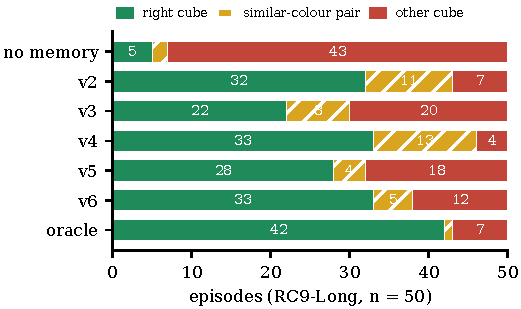
\includegraphics[width=\columnwidth]{figs/fig_errors.pdf}
\caption{Which cube the policy approached on RC9-L (50 episodes): the cue color, the other member of a pair the captioner names alike (red/maroon, yellow/orange, cyan/teal), or another cube.}
\label{fig:errors}
\end{figure}
\begin{table}[!t]
\caption{Test-time note swaps on RC9-L (50 episodes): the policy is fixed and only the note writer changes. Right / pair / other as in Fig.~\ref{fig:errors}. $^\dagger$The disappeared-cue color is replaced by another candidate color; 19 episodes approach the true cube, 14 the named wrong cube, and 17 neither. The pair/other split was not reported for this intervention.}
\label{tab:swap}
\begin{center}
{\footnotesize
\setlength{\tabcolsep}{4pt}
\resizebox{\columnwidth}{!}{%
\begin{tabular}{llcc}
\hline
Trained with & Tested with & Success & Right / pair / other \\
\hline
v4 & v4 & 0.54 & 33 / 13 / 4 \\
v4 & v3 (+ appeared content) & 0.30 & 17 / 9 / 24 \\
v3 & v3 & 0.38 & 22 / 8 / 20 \\
v3 & v4 (removes it) & 0.46 & 27 / 9 / 14 \\
\hline
v6 & no notes & 0.08 & 8 / 2 / 40 \\
v6 & wrong cue color$^\dagger$ & 0.34 & 19 / -- / -- \\
v6 & true cue color & 0.60 & 34 / 7 / 9 \\
\hline
\end{tabular}}
}
\end{center}
\end{table}
v3 notes record both sides of every change. When the candidates appear, the note lists all nine candidate colors (\note{Change: a wooden surface -> a red cube, a green cube, \dots}), so the instruction contains every color word at the moment of the decision.
Removing this appeared content (v4) reduces approaches to unrelated cubes from 20 to 4 of 50 (Fig.~\ref{fig:errors}).
The intervention establishes sensitivity to the note-writer configuration for a fixed policy (Table~\ref{tab:swap}): adding the appeared content at test time to the v4 policy lowers its success from 0.54 to 0.30 (paired difference $-0.24$, 95\% bootstrap interval [$-0.40$, $-0.06$]). Removing it from the v3 policy raises the point estimate from 0.38 to 0.46, but its interval includes zero ($+0.08$, [$-0.08$, $+0.24$]).
Since v3 and v4 also differ in sentence form, the swap measures the joint effect of content and format.

\subsection{Representation}
With v4, 13 of 50 episodes end at the cube that forms a similar-color pair with the cue; both captioners call maroon ``red'' and orange ``yellow'', so the note cannot separate them.
The v6 configuration, which combines measured color names with retention of only the first described object, reduces these confusions to 5. The experiment therefore does not isolate color normalization from object truncation, and total target-choice accuracy remains 33/50 for both v4 and v6.
The finer CSS vocabulary (v5) also reduced pair confusions (4/50) but introduced different names for the same color in the demonstrations and in online rollouts (for example ``blue'' and ``mediumblue''), and approaches to unrelated cubes rose to 18.
A representation must therefore be both discriminative for the task and stable between training and deployment.

\subsection{Utilization}
v6 reduces pair confusions without improving total target-choice accuracy: in all 17 episodes with an incorrect target, the cue note names the correct color.
Many errors involve blue, aqua, and teal, for which the initial scene note can conflict with the measured disappearance note.
However, removing the scene note at test time does not consistently help: the 26-task v6 policy's single-cue mean changes from 0.362 to 0.338 (Table~\ref{tab:long}).
Training without it (v7) reduces this mean to 0.249 and the 26-task mean from 0.145 to 0.097.
The initial note may therefore assist training, but its role is not isolated by these experiments.

Content swaps establish sensitivity to the disappearance note.
Replacing its color with another candidate color reduces success from 0.96/0.94/0.48 to 0.44/0.64/0.34 on RC3/5/9-L.
Among episodes whose closest target is incorrect, the target matches the injected color in 22/22, 15/15, and 14/31 episodes, respectively.
The unchanged scene note is one possible source of retained correct choices; observation biases or other policy behavior may also contribute.
Removing all notes lowers the same policy to 0.26/0.10/0.08.

Correcting the online disappearance color yields 0.90/0.94/0.60, compared with 0.96/0.98/0.80 for the separately oracle-trained policy in these 50-episode evaluations.
On RC9-L, this 12-point gain is descriptively about a third of the 32-point gap.
It is not an additive causal decomposition: oracle training also changes conditioning and note format.
In the oracle policy's 50 episodes, seven closest targets are unrelated cubes and two correct-target episodes do not complete the touch; its extended 150-episode success is 0.87.
Correct information is thus insufficient for reliable action.
These failures are consistent with a grounding limitation, but do not distinguish it from attention, visual recognition, action learning, or execution errors.

\subsection{Memory types across 26 long-horizon tasks}
\begin{table*}[!t]
\caption{Success on the 26 \texttt{-Long} tasks (one joint policy per method, 50 episodes per task). All at 45k steps of the same 90k schedule. $^\dagger$The v6 policy evaluated with v7 notes (scene note at $t{=}0$ removed at test time only). v7: trained and evaluated without the scene note. $^\ddagger$Full frames at our events tiled into an extra image (RePlanMem-style); evaluated on the nine single-cue tasks only.}
\label{tab:long}
\begin{center}
{\footnotesize
\setlength{\tabcolsep}{3pt}
\resizebox{\textwidth}{!}{%
\begin{tabular}{llccccc}
\hline
Family (memory type) & Variants & No memory & Notes v6 & v6, no scene note$^\dagger$ & Notes v7 & Keyframes$^\ddagger$ \\
\hline
RememberColor (object) & 3 / 5 / 9 & .22 / .06 / .04 & .74 / .68 / .28 & .80 / .54 / .30 & .58 / .50 / .38 & .10 / .06 / .06 \\
RememberShape (object) & 3 / 5 / 9 & .20 / .12 / .16 & .38 / .26 / .16 & .32 / .18 / .12 & .18 / .08 / .08 & .14 / .12 / .08 \\
ShapeAndColor (object) & 3x2 / 3x3 / 5x3 & .08 / .06 / .12 & .32 / .26 / .18 & .32 / .32 / .14 & .20 / .20 / .04 & .04 / .06 / .04 \\
BunchOfColors (capacity) & 3 / 5 / 7 & .00 / .00 / .00 & .00 / .00 / .00 & .00 / .00 / .00 & .00 / .00 / .00 & -- \\
SeqOfColors (capacity) & 3 / 5 / 7 & .00 / .00 / .00 & .00 / .00 / .00 & .00 / .00 / .00 & .00 / .00 / .00 & -- \\
ChainOfColors (sequential) & 3 / 5 / 7 & .00 / .00 / .00 & .00 / .00 / .00 & .00 / .00 / .00 & .00 / .00 / .00 & -- \\
ShellGame (tracking) & Touch / Lamp & .20 / .14 & .16 / .26 & .12 / .28 & .08 / .16 & -- \\
BlinkCount (temporal) & E / M / H & .02 / .00 / .00 & .06 / .04 / .00 & .02 / .02 / .00 & .02 / .00 / .00 & -- \\
TimedTransfer (temporal) & E / M / H & .00 / .04 / .06 & .00 / .00 / .00 & .00 / .00 / .00 & .00 / .00 / .02 & -- \\
\hline
Mean (26 tasks) & & 0.058 & 0.145 & 0.134 & 0.097 & -- \\
Mean (9 single-cue tasks) & & 0.118 & 0.362 & 0.338 & 0.249 & 0.078 \\
\hline
\end{tabular}}
}
\end{center}
\end{table*}
Table~\ref{tab:long} reports one policy trained jointly on all 26 tasks with and without notes.
Without memory, $\pi_{0.5}$ reaches 0.058 on average; with notes it reaches 0.145. The representation ablations are compared at a common intermediate 45k-step checkpoint of the same 90k learning-rate schedule, because these runs stop at 45k. The no-memory and v6 runs additionally reach 90k, where their means are 0.048 and 0.116 (single-cue means: 0.076 and 0.298). Thus the final-checkpoint improvement is smaller than the intermediate-checkpoint improvement; the 45k table must not be interpreted as a final-checkpoint comparison.
Benefits concentrate on the nine single-cue object tasks: colors, shapes, and their combinations (mean 0.36 versus 0.12 at equal steps; higher on eight of nine and equal on RememberShape9). On the other 17 tasks both policies stay near zero (0.03 each).
They do not help tasks that require several cues at once (BunchOfColors, SeqOfColors) or in order (ChainOfColors).
For ChainOfColors3 we had verified separately that even the true color sequence in the instruction yields 0/50, showing that correct sequence information alone was insufficient for that policy and task. This single-task control does not establish the failure mechanism for the whole family.
In tracking tasks (ShellGame) the shuffle is a continuous motion of objects that remain visible, which our event trigger does not describe; in BlinkCount each blink produces a note but the window of eight notes truncates long sequences; and in TimedTransfer the frequent lamp and object changes produce about 97 events per episode, most of which are noise.
Across memory types at the same 45k steps, only text notes help: on the nine single-cue tasks the no-memory policy reaches 0.118, keyframes 0.078, v7 notes 0.249, and v6 notes 0.362. The keyframe memory receives the cue frame, written at the same events as the notes, yet stays at or below the no-memory level on eight of the nine tasks (RC9-L: 0.06 versus 0.04), consistent with the absence of a visual-memory benefit in Table~\ref{tab:rc}. Tiling and downsampling may reduce cue readability, so this comparison cannot establish an intrinsic advantage of language over visual memory.

\subsection{Comparison on short RememberColor}
\begin{table}[!t]
\caption{Success on the short RememberColor3/5/9-VLA tasks. Ours: one joint policy per row, 10k steps, 50 episodes per task, GPU physics. $\mu$VLA rows are taken from~\cite{muvla} (OpenVLA-OFT backbone, 100 episodes, trained on a five-task mixture that contains RC5 only, so RC3 and RC9 are held out); the MIKASA-Robo-VLA reference reports RC5 only~\cite{mikasavla}.}
\label{tab:short}
\begin{center}
{\footnotesize
\setlength{\tabcolsep}{4pt}
\resizebox{\columnwidth}{!}{%
\begin{tabular}{lccc}
\hline
Method & RC3 & RC5 & RC9 \\
\hline
$\pi_{0.5}$~\cite{mikasavla} & -- & 0.25 & -- \\
$\pi_{0.5}$~\cite{muvla} & 0.07 & 0.12 & 0.05 \\
OpenVLA-OFT~\cite{muvla} & 0.00 & 0.04 & 0.03 \\
$\mu$VLA ($m{=}64$, $K{=}2$)~\cite{muvla} & 0.92 & 0.93 & 0.41 \\
OpenVLA-OFT + 1st frame~\cite{muvla} & 0.91 & 0.96 & 0.47 \\
\hline
$\pi_{0.5}$ (ours) & 0.30 & 0.18 & 0.10 \\
$\pi_{0.5}$ + event notes v6 (ours) & 0.66 & 0.64 & 0.32 \\
$\pi_{0.5}$ + oracle note (ours) & 0.68 & 0.64 & 0.64 \\
\hline
\end{tabular}}
}
\end{center}
\end{table}
On these short tasks, only the initial scene note is written; there is no disappearance event to select.
It raises success from 0.30/0.18/0.10 to 0.66/0.64/0.32, approaching the oracle reference on RC3/5 but leaving a larger RC9 gap (Table~\ref{tab:short}).
The oracle reference itself reaches only 0.68/0.64/0.64, indicating limitations beyond generated-note accuracy.
The higher RC3/5 results of $\mu$VLA and first-frame memory come from different backbones, training mixtures, and episode counts; they provide context, not a controlled ranking.
The Long tasks test retention beyond a first-frame caption, but our experiments do not establish that disappearance notes are the only suitable memory.
\begin{table}[!t]
\caption{Success on the standard MIKASA-Robo RememberColor3/5/9-v0 tasks~\cite{mikasa} (250 demonstrations per task; ours with 100 evaluation episodes per task). External numbers are taken from the cited papers; their action spaces, backbones, and checkpoint selection differ (see text). Ours: one joint policy per row, fixed 10k-step checkpoint, joint-delta actions, the -VLA instruction text added.}
\label{tab:v0}
\begin{center}
{\footnotesize
\setlength{\tabcolsep}{4pt}
\resizebox{\columnwidth}{!}{%
\begin{tabular}{lccc}
\hline
Method & RC3 & RC5 & RC9 \\
\hline
MemoryVLA~\cite{memoryvla} & 0.44 & 0.30 & 0.20 \\
MemoryVLA++~\cite{memoryvlapp} & 0.50 & 0.19 & 0.16 \\
SimpleMemVLA~\cite{simplememvla} & 0.71 & 0.58 & 0.59 \\
GMP~\cite{gmp} & 0.80 & 0.61 & 0.17 \\
Chameleon~\cite{chameleon} & 0.94 & 0.72 & 0.53 \\
\hline
$\pi_{0.5}$ (ours) & 0.19 & 0.14 & 0.14 \\
$\pi_{0.5}$ + event notes v6 (ours) & 0.65 & 0.84 & 0.51 \\
\hline
\end{tabular}}
}
\end{center}
\end{table}
On standard RememberColor-v0, notes raise success from 0.19/0.14/0.14 to 0.65/0.84/0.51 (Table~\ref{tab:v0}); again, the memory is a single initial scene caption.
These values overlap the range of published results, but protocols differ.
GMP trains per task; Chameleon uses a small non-VLA policy and 30 episodes over three seeds; MemoryVLA, MemoryVLA++, and GMP report best checkpoints.
Their action spaces also differ from our joint-delta actions.
The table therefore contextualizes absolute success without establishing superiority or parity with architectural memory.

\subsection{Discussion and limitations}
The strongest evidence is for single-cue recall under matched policy-training conditions, with interpretable interventions on the instruction memory.
Several limitations constrain broader claims.
First, each configuration uses one training seed. Episode-level and paired-bootstrap confidence intervals cannot establish robustness to optimization randomness.
Second, the coarse color measurement is designed for rendered attributes; it does not validate performance under real camera noise, lighting variation, or multi-object changes. Retaining one object and eight notes also imposes explicit capacity limits.
Third, note variants change multiple factors, including captioner size, wording, and object truncation. Their differences are diagnostic configurations rather than fully isolated component ablations.
Fourth, the visual baseline uses a compressed tiled image and a different input interface, while external methods use different training and evaluation protocols.
Fifth, the stationarity assumption and CPU physics constrain transfer to continuously moving robots and canonical GPU evaluation. The eight replay episodes motivate the backend choice but do not establish a benchmark-wide physics failure.
Finally, no inference-latency, total-compute, or real-robot evaluation is provided. The architecture is unchanged, but the captioner adds computation and the policy still requires memory-conditioned fine-tuning.
Periodic captioning, matched first-frame memory on the Long tasks, repeated training seeds, and event precision/recall would strengthen attribution of the benefit to event-driven selection.

%======================================================================
\section{CONCLUSION}
%======================================================================
Short external language notes substantially improve a fine-tuned, current-observation VLA on single-cue long-horizon manipulation tasks without changing its architecture.
Fixed-policy interventions show sensitivity to the notes, while target-choice diagnostics distinguish captioning errors from failures despite correct cue descriptions.
Selection and representation changes alter error patterns, but do not eliminate the gap to separately oracle-conditioned policies.
The benefit does not extend consistently to multi-cue, tracking, counting, or timing tasks in our custom 26-task evaluation.
These findings support language notes as an interpretable memory interface for single-cue recall and motivate richer memory and grounding mechanisms for broader partial observability.

%======================================================================
\section*{DECLARATIONS}
\subsection*{Conflict of Interest}
The authors declare that there is no competing financial interest or personal relationship that could have appeared to influence the work reported in this paper.
\subsection*{Authors' Contributions}
\tbd{}
\subsection*{Funding}
\tbd{}
\subsection*{Data Availability}
\tbd{Code, note datasets, and evaluation logs: repository link.}
\subsection*{Use of AI Tools}
% Required by IJCAS: immediately before the References. Fill in truthfully.
OpenAI Codex was used to assist with manuscript editing, consistency checks between the manuscript and implementation, and statistical summaries of existing evaluation logs. The authors remain responsible for verifying all claims, calculations, references, and manuscript content.

%======================================================================
% References: titles and author metadata checked against primary sources, 2026-11-05.
\begin{reference}
\bibitem{pi05} Physical Intelligence et al., ``$\pi_{0.5}$: A vision-language-action model with open-world generalization,'' \textit{arXiv preprint} arXiv:2504.16054, 2025.
\bibitem{lerobot} R. Cadene et al., ``LeRobot: State-of-the-art machine learning for real-world robotics in PyTorch,'' [Online]. Available: https://github.com/huggingface/lerobot, 2024.
\bibitem{smolvlm} A. Marafioti et al., ``SmolVLM: Redefining small and efficient multimodal models,'' \textit{arXiv preprint} arXiv:2504.05299, 2025.
\bibitem{mikasa} E. Cherepanov, N. Kachaev, A. K. Kovalev, and A. I. Panov, ``Memory, benchmark \& robots: A benchmark for solving complex tasks with reinforcement learning,'' \textit{Proc. of International Conference on Learning Representations (ICLR)}, 2026.
\bibitem{mikasavla} E. Cherepanov, N. Kachaev, A. I. Panov, and A. K. Kovalev, ``MIKASA-Robo-VLA: Benchmarking memory in VLA models for long-horizon manipulation,'' \textit{arXiv preprint} arXiv:2610.00604, 2026.
\bibitem{replanmem} V. Smelova et al., ``When Plans Change, Remember: Replanning-Guided Visual Memory for Vision-Language-Action Models,'' \textit{arXiv preprint} arXiv:2610.22556, 2026.
\bibitem{muvla} E. Cherepanov et al., ``$\mu$VLA: On Recurrent Memory for Partially Observable Manipulation in VLA Models,'' \textit{arXiv preprint} arXiv:2606.12497, 2026.
\bibitem{robomme} Y. Dai et al., ``RoboMME: Benchmarking and understanding memory for robotic generalist policies,'' \textit{Proceedings of Machine Learning Research}, vol. 306, pp. 22396--22450, 2026.
\bibitem{memoryvla} H. Shi et al., ``MemoryVLA: Perceptual-Cognitive Memory in Vision-Language-Action Models for Robotic Manipulation,'' \textit{arXiv preprint} arXiv:2508.19236, 2025.
\bibitem{memoryvlapp} H. Shi et al., ``MemoryVLA++: Temporal Modeling via Memory and Imagination in Vision-Language-Action Models,'' \textit{arXiv preprint} arXiv:2606.09827, 2026.
\bibitem{simplememvla} C. Yin et al., ``SimpleMemVLA: A Simple but Effective Native-Video Memory for Vision-Language-Action Models,'' \textit{arXiv preprint} arXiv:2609.05533, 2026.
\bibitem{gmp} Y. Gao, J. J. Liu, S. Li, and S. Song, ``Gated Memory Policy: In-Context Memorization and Adaptation,'' \textit{arXiv preprint} arXiv:2604.18933, 2026.
\bibitem{chameleon} X. Guo et al., ``Chameleon: Control-Indexed Prospective Memory for Visuomotor Manipulation,'' \textit{arXiv preprint} arXiv:2603.24576, 2026.
\end{reference}

\end{document}
